%% Adaptado de 
%% http://www.ctan.org/tex-archive/macros/latex/contrib/IEEEtran/
%% Traduzido para o congresso de IC da USP
%%*****************************************************************************
% Não modificar

\documentclass[twoside,conference,a4paper]{IEEEtran}

%******************************************************************************
% Não modificar
\usepackage{IEEEtsup} % Definições complementares e modificações.
\usepackage[utf8]{inputenc} % Disponibiliza acentos.
\usepackage[english]{babel}
%% Disponibiliza Inglês e Português do Brasil.
\usepackage{latexsym,amsfonts,amssymb} % Disponibiliza fontes adicionais.
\usepackage{theorem} 
\usepackage[cmex10]{amsmath} % Pacote matemático básico 
\usepackage{url} 
\usepackage{graphicx}
\usepackage{amsmath}
\usepackage{amssymb}
\usepackage{color}
\usepackage[pagebackref=true,breaklinks=true,letterpaper=true,colorlinks,bookmarks=false]{hyperref}
\usepackage[tight,footnotesize]{subfigure} 
\usepackage[noadjust]{cite} % Disponibiliza melhorias em citações.
\usepackage{tikz}
\newcommand*\circled[1]{\tikz[baseline=(char.base)]{
            \node[shape=circle,draw,inner sep=1pt] (char) {#1};}}
%%*****************************************************************************

\usepackage{listings}
\lstset{basicstyle=\footnotesize\ttfamily,  language=Python}
\renewcommand{\lstlistingname}{Code}% Listing -> Algorithm

\begin{document}
\renewcommand{\IEEEkeywordsname}{Palavras-chave}

%%*****************************************************************************

\urlstyle{tt}
% Indicar o nome do autor e o curso/nível (grad-mestrado-doutorado-especial)
\title{P2 - Simulador Robótico}
\author{%
 \IEEEauthorblockN{Isadora Sophia Garcia Rodopoulos\,\IEEEauthorrefmark{1}\\
                   Renato Landim Vargas\,\IEEEauthorrefmark{1}}
 \IEEEauthorblockA{\IEEEauthorrefmark{1}%
                   Ciência da Computação - Graduação - RA 158018\\
                   E-mail: ra158018@ic.unicamp.br}
 \IEEEauthorblockA{\IEEEauthorrefmark{1}%
                   Ciência da Computação - Graduação - RA 118557\\
                   E-mail: ra118557@ic.unicamp.br}
}

%%*****************************************************************************

\maketitle

%%*****************************************************************************
% Resumo do trabalho
\begin{abstract}
O trabalho se baseou em implementar assuntos teóricos desenvolvidos em sala de aula,
entre eles: explorar métodos de controle mais avançados e computar a odometria
do robô através de um modelo cinemático. Os assuntos são desenvolvidos a partir de
um ambiente com o robô p3dx, com o suporte do \textit{V-REP}.

O objetivo se trata de fazer o robô explorar o cenário e coletar informações relevantes tanto sobre o ambiente quanto sua localização. A solução foi proposta através do mapeamento de informações com o Ground Trouth, com o auxílio de gráficos, e utilizando o modelo cinemático com a odometria para o controle do robô. Para tornar o controle mais robusto, foi utilizado métodos como o sistema \textbf{fuzzy}, para que o robô possa acompanhar as paredes, desviar de obstáculos, além de uma subrotina para evitar que fique preso.

O resultado foi um sistema de controle mais robusto com sensores que se assemelham mais a uma situação do mundo real - isto é, sem a utilização de Ground Trouth para se locomover.

% O resumo deve conter uma breve descrição sobre várias partes do seu trabalho que serão tratadas no decorrer do texto. Primeiramente, pode-se descrever brevemente o problema no qual você está trabalhando: Por que você está desenvolvendo este trabalho? Qual a motivação para este desenvolvimento? Por que ele é importante? O resumo deve conter também um breve descritivo da metodologia que você usou no desenvolvimento: Que problema foi tratado? Como a solução foi construída/desenvolvida? Quais as tecnologias utilizadas? Finalmente, deve falar um pouco sobre os resultados que você conseguiu: o resultado final ficou bom? Quais os seus principais diferenciais? Qual a eficiência do desenvolvimento?

\end{abstract}

\begin{IEEEkeywords}
fuzzy, odometria, sistemas inteligentes.

% Indique três palavras-chave que descrevem o trabalho

\end{IEEEkeywords}

%%*****************************************************************************

\section{Introdução}
O projeto foi baseado na literatura proposta em sala de aula e em papers relacionados ao problema proposto, o qual o sistema fuzzy foi baseado \cite{Reinhard:1995}. O foco do projeto se deu à aproximação da simulação com problemas do mundo real, com a introdução de odometria e controladores mais robustos, com foco em sistemas fuzzy.

Apesar de sistemas fuzzy serem menos utilizados no estado da arte da robótica atual, há vários trabalhos de anos anteriores que o utilizam para a resolução de problemas. Além disso, ainda é um conceit obastante utilizado para a programação de uma AI em videogames, por exemplo, devido a seu baixo custo computacional.

O trabalho encontra-se organizado da seguinte forma: a seção 2, descrevendo o modelo cinemático utilizado; a seção 3, descrevendo o processo realizado para a odometria; a seção 4, apresentando os estados de controle do robô; os resultados são apresentados na seção 5 e, finalmente, as conclusões são apresentadas na seção 6. \textbf{(não sei se vai ser isso?? acho que não)}

% Na introdução você deve descrever os aspectos mais relevantes sobre a revisão bibliográfica que fez e do problema que você decidiu tratar. Quais foram os pontos estudados/pesquisados? Quais os outros trabalhos similares ao seu que você encontrou? 

% Também na introdução espera-se que você descreva um pouco sobre a motivação de trabalhar com esse tema. A descrição do seu trabalho será feita em detalhes nas próximas seções do artigo.

% No final da introdução, é comum inserir um parágrafo descrevendo o que será encontrado em cada seção no restante do seu texto. Exemplo: Este trabalho encontra-se organizado da seguinte forma: a seção 2 apresenta X. A seção 3 descreve Y. Os resultados são apresentados na seção 4, e as conclusões são apresentadas na seção 5.

\section{Modelo cinemático}

O modelo cinemático do robô utilizado foi o diferencial. Para isso, é necessário calcular a velocidade linear de cada uma das duas rodas, $V_{r}$ (roda direita) e $V_{l}$ (roda esquerda). Esses dois valores são calculados da seguinte forma:
\begin{gather*}
V_{r} = r * \phi_{r} \\
V_{l} = r * \phi_{l},
\end{gather*}
onde $r$ é o raio da roda e $\phi_{r}$ e $\phi_{l}$ são as velocidades angulares de cada roda. Essas velocidades são calculadas através das diferenças de posição angulares das rodas em um certo $\Delta t$, dividindo a variação angular pela variação de tempo.

Então, calcula-se as velocidades linear e angular do robô da seguinte forma:
\begin{gather*}
V = \frac{V_{r} + V_{l}}{2} \\
\omega = \frac{V_{r} - V_{l}}{2 * L},
\end{gather*}
onde L é metade da distância entre as rodas. A partir dessas duas velocidades, calcula-se a variação de distância e ângulo para uma certa variação de tempo. 
\begin{gather*}
\Delta s = V * \Delta t \\
\Delta \theta = \omega * \Delta t
\end{gather*}
Com essas variações, pode-se somar à posição atual para calcular uma posição nova.

\subsection{Sistema de referência}

Como o robô calcula apenas variações de posição e ângulo, ele não sabe sua posição exata no mundo, mas apenas no seu sistema de referência local. Para converter essa posição local para uma posição no mundo, foi implementado um conversor entre modelos de referências. Esse conversor cria e salva as matrizes de rotação e translação para converter a qualquer momento. Porém, para que isso seja possível, é necessário inserir a posição inicial do robô no mundo.

\section{Odometria}

Como não era permitido usar o ground truth do robô e os resultados do modelo cinemático básico são insatisfatórios, foi necessário calcular a sua odometria para estimar uma variação de pose mais precisa. Para um certo frame $t$, pode-se calcular essa variação por:
\begin{gather*}
\Delta \xi_{t} =
\begin{bmatrix}
\Delta s * \cos(\theta_{t-1} + \frac{\Delta \theta_{t}}{2}) \\
\Delta s * \sin(\theta_{t-1} + \frac{\Delta \theta_{t}}{2}) \\
\theta_{t}
\end{bmatrix}
\end{gather*}
Somando essa variação a cada frame, obtemos um valor de pose mais próximo da realidade comparado ao anterior.

\subsection{Correção}

Apesar de obter-se resultados melhores com a odometria, a variação de ângulo ainda é muito imprecisa e propaga muitos erros. Para um valor mais preciso, utilizou-se um giroscópio. O giroscópio originalmente retorna apenas variações de ângulo, mas como não pode-se garantir que será possível ler  o giroscópio sempre que dados novos aparecerem, ele foi modificado para somar essas variações e sempre retornar a sua estimativa de posição angular. As equações de odometria não mudam, mas apenas utilizam o novo valor de $\Delta \theta$.

\section{Sistema de controle}

O sistema de controle foi dividido em dois comportamentos distintos: o Wall Follow, que permite que o robô siga a parede ao mesmo tempo que procura desviar de obstáculos; e o Unstuck, o qual verifica se o robô está preso e, caso afirmativo, o retira desse estado.

\subsection{Wall Follow}

O Wall Follow foi baseado em conjuntos Fuzzy da literatura \cite{Reinhard:1995}. Basicamente, foram utilizadas duas regras: \textbf{directional} e \textbf{speed}, que regula a direção e a velocidade do robô. Os inputs e as regras de  defuzzification utilizados estão ilustrados nas figuras abaixo.

\begin{figure}[]
  \centering
  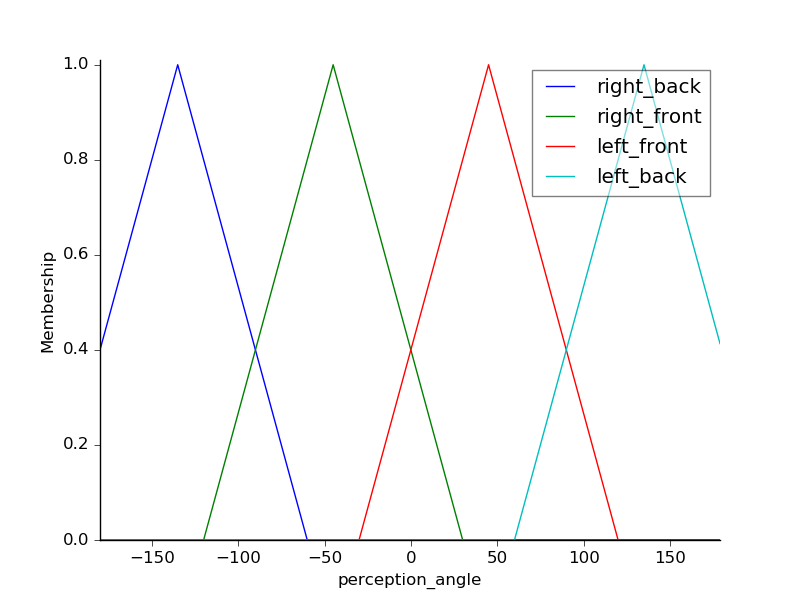
\includegraphics[width=1\hsize]{figuras/per_angle.png}
  \caption{Ângulo em que o robô detectou o obstáculo, ie. parede.}
  \label{fig:fig1}
  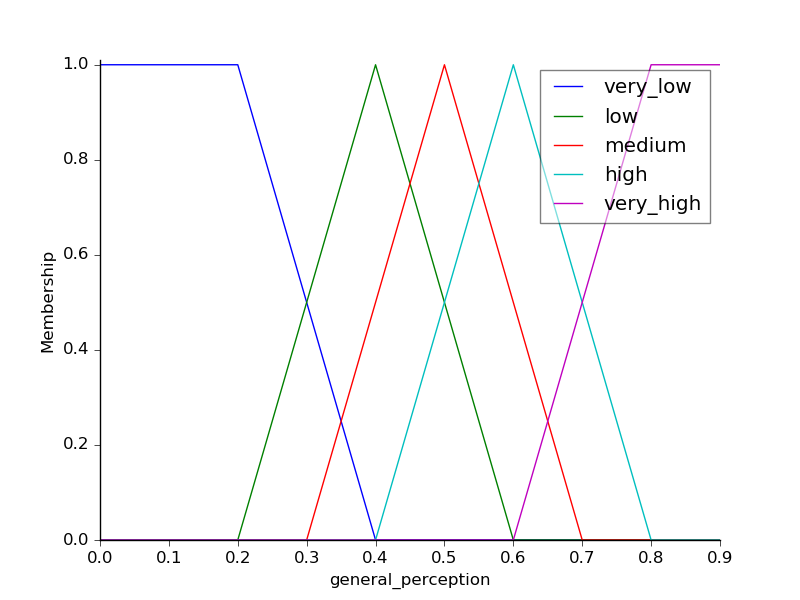
\includegraphics[width=1\hsize]{figuras/per.png}
  \caption{Um exemplo de figura.}
  \label{fig:fig2}
  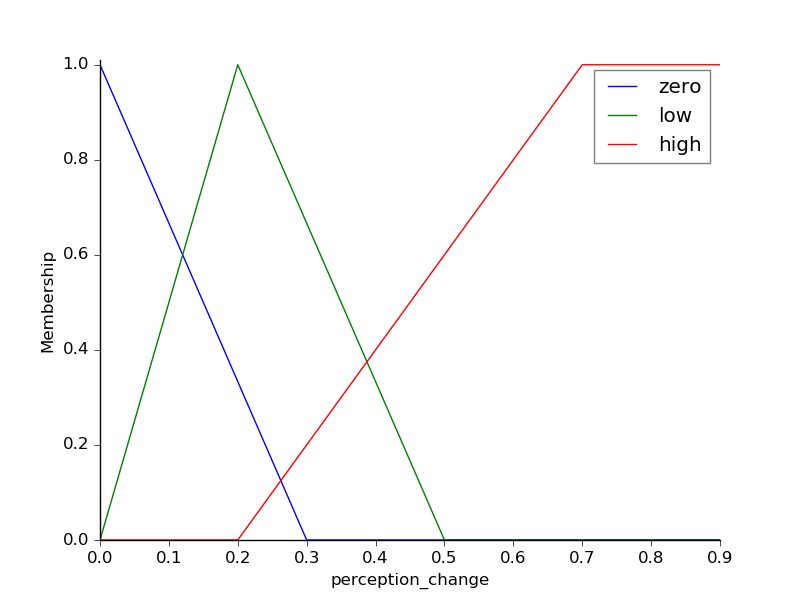
\includegraphics[width=1\hsize]{figuras/per_change.png}
  \caption{Um exemplo de figura.}
  \label{fig:fig3}

  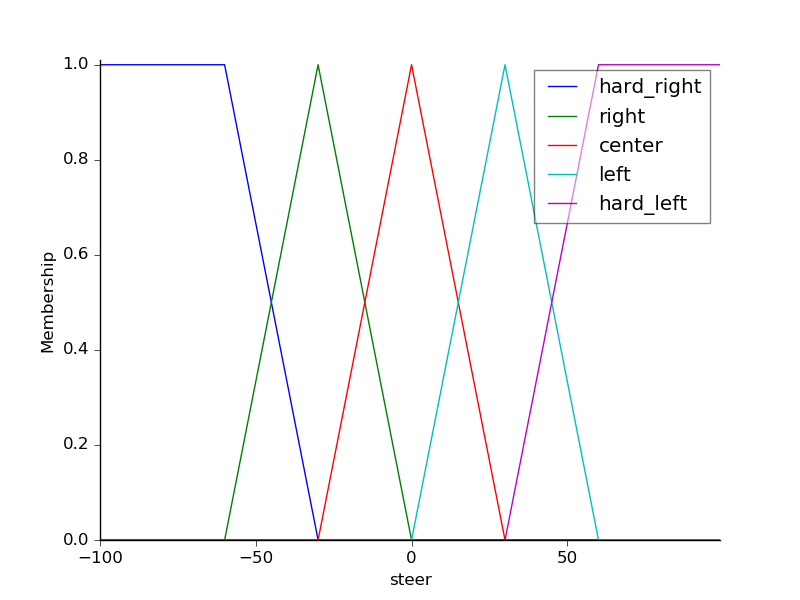
\includegraphics[width=1\hsize]{figuras/steer.png}
  \caption{Um exemplo de figura.}
  \label{fig:fig4}

  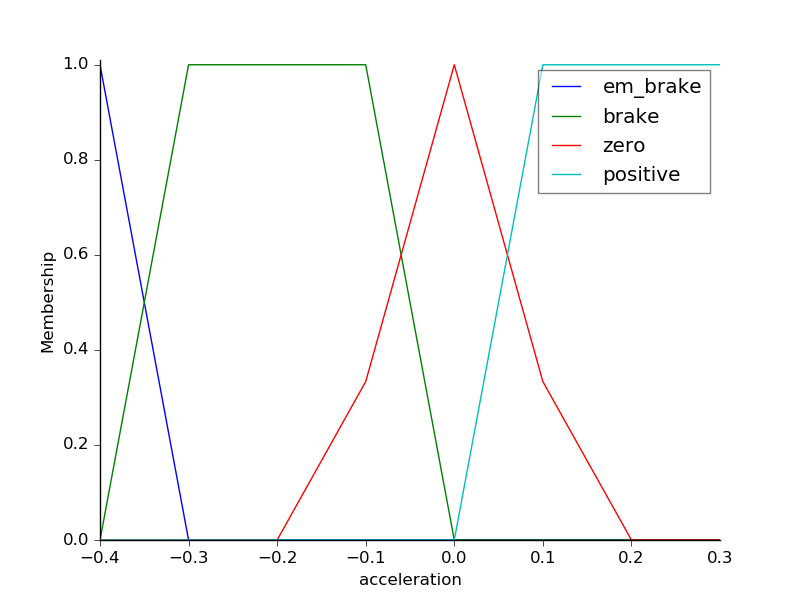
\includegraphics[width=1\hsize]{figuras/acc.png}
  \caption{Um exemplo de figura.}
  \label{fig:fig5}
\end{figure}

Para facilitar a criação de regras e de conjuntos Fuzzy, foi utilizada a biblioteca \texttt{skfuzzy}, de python. Além disso, como os parâmetros dos inputs não eram, necessariamente, adequados para o nosso robô do experimento (devido a fatores como o peso do robô, por exemplo), foram utilizado valores de escala para a velocidade angular $v_{a} = .45$ e para a velocidade linear $v_{l} = 2$. 

Portanto, o algoritmo se baseia na seguinte iteração: \\

  \subsubsection{Encontra valor da magnitude e ângulo do obstáculo mais próximo}
    Para isso, basta encontrar o valor da menor leitura dentre os sensores, e o seu respectivo ângulo. 

    O valor é escalado para que quanto mais perto o objeto, mais próximo de 1 - ou seja, $p = 1-p'$, com $p'$ sendo a leitura mínima do sensor. O valor do ângulo é retornado em graus (dentre $-170^{\circ}$ a $170^{\circ}$). \\

  \subsubsection{Reflete os valores em nossos conjuntos Fuzzy, obtendo velocidade angular e a aceleração da velocidade}
    Para cada uma das duas regras, \textbf{directional} e \textbf{speed}, bastou-se passar os parâmetros obtidos e obter o output da defuzzification. Para obter o valor de \texttt{perception\_change}, basta obter a diferença de percepção em relação a última iteração. O código abaixo ilustra os processos realizados.

    \begin{lstlisting}[caption={Aplicação dos conjuntos fuzzy}]
angle, magnitude = self.get_perception_values()

perception_change = 
      clamp(abs(magnitude-last_magnitude))

# get ANGULAR speed for robot
directional.input['perception_angle'] = angle
directional.input['general_perception'] = magnitude
directional.compute()
v_angular = math.radians(directional.output['steer'])

# get LINEAR speed for robot
speed.input['perception_change'] = perception_change
speed.input['general_perception'] = magnitude
speed.compute()
acc = math.radians(speed.output['acceleration'])
    \end{lstlisting}

  \subsubsection{Verifica se o robô está preso}
  \subsubsection{Atualiza os valores}


\subsection{Unstuck}

\section{Trabalho Proposto}

Nesta seção descreva de forma abrangente, porém clara e organizada, o seu trabalho.

\subsection{Tabelas}

Uma tabela pode ser posicionada em qualquer lugar no texto, como no exemplo
seguinte.
%
\begin{table}[ht]
\renewcommand{\arraystretch}{1.3}
\centering
 \caption{Exemplo de texto de uma tabela.}
 \label{tab:tab1}
 \begin{tabular}{lcccc}\hline
  & \multicolumn{2}{c}{Texto}
  & \multicolumn{2}{c}{Sem \#21} \\ \cline{2-5}
  X & Y & $z$ & $\mathcal{A}$ & valor-$z$ \\ \hline \hline
  1      &0,491  & 3,66   &0,367 &2,46  \\
  2    &0,732  & 4,21   &0,354 &1,50  \\
  3      &0,000  & -      &0,000 & -    \\
  4      &0,000  & -      &0,000 & -  \\
  5      &0,421  & 1,94   &0,668 &2,79  \\
  6      &0,421  & 1,94   &0,668 &2,79  \\
  7      &0,938  & 3,92   &1,295 &4,67 \\
  8       &0,000  & -      &0,000 & - \\
  9       &0,356  & 1,40   &0,491 &1,87 \\ \hline
 \end{tabular}
\end{table}

Para citar esta tabela, em qualquer ponto no texto, como Tabela~\ref{tab:tab1}.


\section{Materiais e Métodos}

Todo trabalho deve ser submetido a algum tipo de teste para que possa ser avaliado. Na verdade, buscamos aqui uma validação com um caráter mais científico de seu trabalho (validação de hipótese). Busca-se identificar quais os seus pontos fortes e fracos. Nesta seção você deve descrever claramente quais foram e como foram conduzidos os testes, quais os materiais e as metodologias empregadas.   

Uma figura pode ser posicionada em qualquer lugar no texto, como no exemplo seguinte da Figura~\ref{fig:plot1}.


Use o comando ``cite'' para citar itens na sua lista de
referências através dos seus rótulos.


\section{Resultados e Discussão}

Para análise dos resultados, foi extraída uma nuvem de pontos representando as posições calculada (em verde) e ground true (em azul) do robô, as posições com obstáculos detectados pelos sonares (em preto), e também as posições onde o robô foi detectado como preso (em vermelho). Um exemplo do código rodando pode ser visto na Figura~\ref{fig:plot1}.

\begin{figure}[ht]
\centering
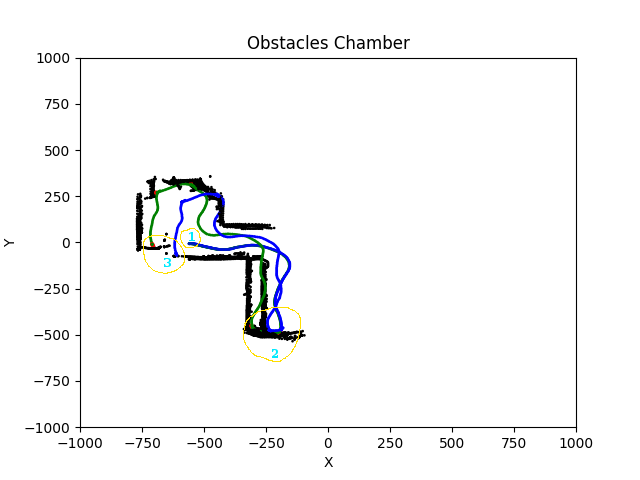
\includegraphics[width=1\hsize]{figuras/figure_3.png}
\caption{Um exemplo de plot gerado. Os círculos amarelos representam momentos a serem discutidos.}
\label{fig:plot1}
\end{figure}

Nesse exemplo, o robô começa sua posição em \circled{1}. Entre esse momento, e o momento \circled{2}, as linhas azul e verdes são indicerníveis por terem um valor muito próximo. Porém nota-se que em \circled{2}, o robô fica preso por um tempo tentando andar através de um obstáculo. Nesse instante, ocorre derrapagem e a posição estimada do robô é comprometida. Isso é notável no caminho até o momento \circled{3}, onde as linhas já estão relativamente separadas. Porém, nota-se que a orientação estimada continua alinhada com a orientação real, não sendo afetada por erros de derrapagem por ser calculada através de um giroscópio.

Nesse exemplo também é possível ver que o robô executando $Wall Follow$ de fato segue paredes, mas em vários momentos esbarra em paredes e fica preso. Nesses momentos, o robô entra em modo $Unstuck$ e eventualmente consegue sair. Porém, devido à tendência de ficar preso, as estimativas de pose do robô tendem a piorar nesses momentos.

\section{Conclusões}

Nesta seção, faça uma análise geral de seu trabalho, levando em conta todo o processo de desenvolvimento e os resultados. Quais os seus pontos fortes? Quais os seus pontos fracos? Quais aspectos de sua metodologia de trabalho foram positivas? Quais foram negativas? O que você recomendaria (ou não recomendaria) a outras pessoas que estejam realizando trabalhos similares aos seus? 


%******************************************************************************
% Referências - Definidas no arquivo relatorio.bib
 +-------------+

\bibliographystyle{IEEEtran}

\bibliography{relatorio}

%******************************************************************************

\end{document}
